% ======================================================================
\section{Comparing institutions}\label{sec:score}
% ======================================================================

Each planner in this paper is a rule for choosing public policies, and so is each of the practices it stands for: keeping what is in force, piloting and then deciding, learning as you go, protecting everyone, taking turns. They can be scored on one card: welfare, each person's gain over the status quo, and the largest conflict loss. We fill in the card for \cref{ex:sq}, first in the long run and then at finite horizons.

\paragraph{The long run.} \Cref{tab:score} gives the policy each institution settles on and what it pays. Every entry is the solution of a linear program.

\begin{table}[h]\centering\small
\begin{tabular}{lcccc}
\toprule
& welfare & \multicolumn{2}{c}{gain over the status quo} & largest\\
institution (long-run policy) & per round & persons 1, 2 & person 3 & conflict loss\\
\midrule
keep the status quo & 2.60 & $0$ & $0$ & 0.80\\
utilitarian learner ($\astar$) & 3.00 & $-0.20$ & $+0.80$ & 0.50\\
utilitarian learner, losers made whole & 3.00 & $0$ & $+0.40$ & --\\
utilitarian learner, surplus shared equally & 3.00 & $+0.13$ & $+0.13$ & --\\
unanimity, $\alpha=0$ ($60\%\ \astar$, $40\%\ b$) & 2.96 & $0$ & $+0.36$ & 0.44\\
tolerance $\alpha=0.05$ ($70\%\ \astar$, $30\%\ b$) & 2.97 & $-0.05$ & $+0.47$ & 0.35\\
smallest largest conflict loss ($69\%\ \astar$, $31\%\ b$) & 2.97 & $-0.04$ & $+0.46$ & 0.34\\
\bottomrule
\end{tabular}
\caption{\Cref{ex:sq}: long-run outcome per round. The two transfer rows are insure-and-share (\cref{def:insure}) with shares $(0,0,1)$ and $(\tfrac13,\tfrac13,\tfrac13)$; they require transferable rewards. The unanimity row is the best outcome that leaves no one worse off; a planner that must also \emph{learn} under $\alpha=0$ never leaves the status quo (\cref{prop:nofree}).}
\label{tab:score}
\end{table}

\paragraph{Finite horizons.} The long-run card leaves out the cost of getting there. For that we run each institution as a planner that starts knowing only the status quo, and record the expected reward it gives each person, averaged over the first $T$ rounds. The planners are:
\begin{itemize}[leftmargin=*,itemsep=1pt]
  \item \emph{keep the status quo}, which is also what a planner bound by unanimity must do;
  \item \emph{adopt $\astar$ at once}, an oracle, for reference;
  \item the \emph{utilitarian learner}: Thompson sampling on the welfare signal, with the status quo's welfare known (UCB behaves similarly and is in the results file);
  \item \emph{pilot, then decide}: try each alternative for $T^{2/3}/(K-1)$ rounds, then keep whichever has the best observed total for the rest of the horizon;
  \item a \emph{time-share} learner, which plays the equal-conflict time-share of \cref{prop:share} computed from current estimates, mixed with uniform exploration of weight $t^{-1/3}$;
  \item the \emph{individually rational} planner of \cref{sec:sq}, with $\alpha=0.05$ and $\alpha=0.2$;
  \item \emph{compensation}: the transfers of \cref{def:insure} with equal shares, on top of the utilitarian learner, and on top of the pooled-floor planner of \cref{sec:comp} with $\alpha=0.05$ and $\alpha=0.2$.
\end{itemize}
The pilot length and the exploration weights are not tuned. \Cref{fig:score,tab:scoreT} report the results.

\begin{figure}[t]\centering
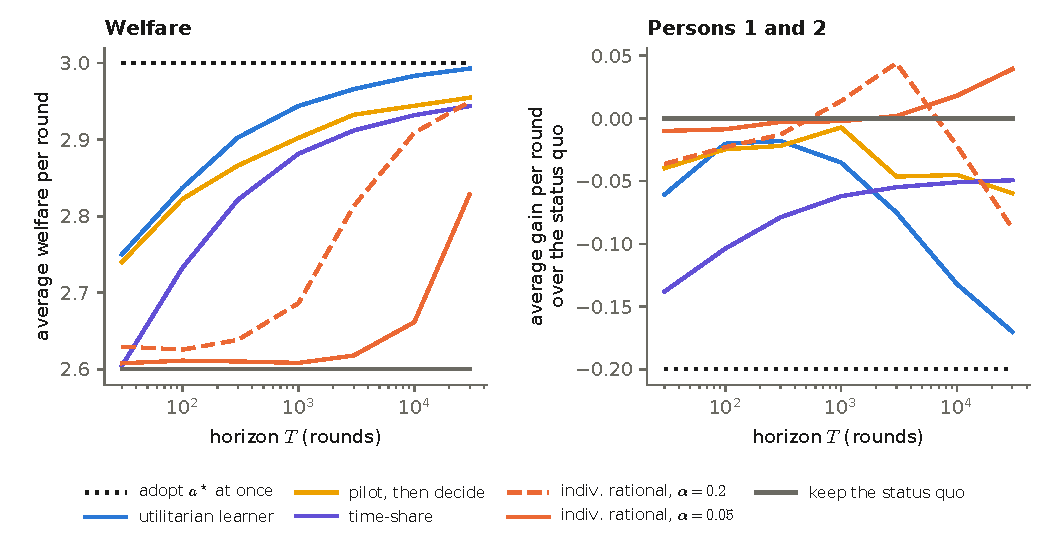
\includegraphics[width=\linewidth]{figures/fig_scorecard.pdf}
\caption{\Cref{ex:sq}: seven institutions without transfers at horizons from $30$ to $30{,}000$ rounds. Left: welfare per round, averaged over the horizon. Right: the average gain of persons 1 and 2, whom the status quo favours. Means over 200 runs (40 for the time-share and individually rational planners).}
\label{fig:score}
\end{figure}

\begin{table}[h]\centering\small
\begin{tabular}{l ccc ccc ccc}
\toprule
& \multicolumn{3}{c}{$T=30$} & \multicolumn{3}{c}{$T=1{,}000$} & \multicolumn{3}{c}{$T=30{,}000$}\\
institution & $W$ & $G_{1,2}$ & $G_3$ & $W$ & $G_{1,2}$ & $G_3$ & $W$ & $G_{1,2}$ & $G_3$\\
\midrule
keep the status quo & 2.60 & $0$ & $0$ & 2.60 & $0$ & $0$ & 2.60 & $0$ & $0$\\
adopt $\astar$ at once & 3.00 & $-.20$ & $+.80$ & 3.00 & $-.20$ & $+.80$ & 3.00 & $-.20$ & $+.80$\\
utilitarian learner & 2.75 & $-.06$ & $+.27$ & 2.94 & $-.04$ & $+.41$ & 2.99 & $-.17$ & $+.73$\\
pilot, then decide & 2.74 & $-.04$ & $+.22$ & 2.90 & $-.01$ & $+.32$ & 2.96 & $-.06$ & $+.47$\\
time-share & 2.61 & $-.14$ & $+.28$ & 2.88 & $-.06$ & $+.41$ & 2.94 & $-.05$ & $+.44$\\
individually rational, $\alpha=0.2$ & 2.63 & $-.04$ & $+.10$ & 2.69 & $+.01$ & $+.06$ & 2.95 & $-.09$ & $+.53$\\
individually rational, $\alpha=0.05$ & 2.61 & $-.01$ & $+.03$ & 2.61 & $-.00$ & $+.01$ & 2.83 & $+.04$ & $+.15$\\
\midrule
utilitarian learner, compensated & 2.75 & $+.05$ & $+.05$ & 2.94 & $+.11$ & $+.11$ & 2.99 & $+.13$ & $+.13$\\
compensation, pooled floor, $\alpha=0.2$ & 2.64 & $+.01$ & $+.01$ & 2.86 & $+.09$ & $+.09$ & 2.96 & $+.12$ & $+.12$\\
compensation, pooled floor, $\alpha=0.05$ & 2.61 & $+.00$ & $+.00$ & 2.66 & $+.02$ & $+.02$ & 2.96 & $+.12$ & $+.12$\\
\bottomrule
\end{tabular}
\caption{\Cref{ex:sq}: welfare per round $W$ and average gain over the status quo for persons 1 and 2 ($G_{1,2}$) and person 3 ($G_3$), averaged over the first $T$ rounds. The last three rows use the transfers of \cref{def:insure} with equal shares. Standard errors of $W$ are at most $0.02$ at $T=30$ and $0.01$ at the longer horizons.}
\label{tab:scoreT}
\end{table}

Four things stand out.

\emph{Learning at all matters more than how.} At $T=30$ the utilitarian learner and the pilot both reach about $2.75$, against $2.60$ for the status quo and $3.00$ for the oracle. The gap between them is small next to the gap between either and doing nothing.

\emph{The cost to the people the status quo favours arrives late.} Under the utilitarian learner, persons 1 and 2 lose $0.02$ to $0.06$ per round at horizons up to $1{,}000$, and $0.17$ at $30{,}000$. Early on the learner spends much of its time on $b$, which they prefer; as it becomes sure of $\astar$ it stops. At short horizons a utilitarian learner behaves like a time-share without intending to.

\emph{Compensation is affordable at every horizon.} Holding persons 1 and 2 at their status-quo level under the utilitarian learner would take transfers of between $0.04$ and $0.34$ per round, depending on the horizon. That is between $12\%$ and $87\%$ of the welfare the learner gains over the status quo, and never more than it. With the surplus shared equally, everyone is above the status quo in expectation at each of the horizons we ran.

\emph{A guarantee is expensive in time, tolerance buys speed, and pooling buys more.} With $\alpha=0.05$ the individually rational planner gains almost nothing for $10^4$ rounds; by $30{,}000$ it has everyone above the status quo, at welfare $2.83$. With $\alpha=0.2$ it has everyone above the status quo by $3{,}000$ rounds. With compensation and a pooled floor at $\alpha=0.05$, welfare is $2.96$ at $30{,}000$ rounds and everyone gains from the first round (\cref{sec:comp}). A collective that insists on a tight per-person guarantee without transfers and has a short horizon gets, in effect, the status quo.

These are expectations on one example with three people, and the ranking will change with the instance. What the exercise shows is that the institutions can be compared on common terms, and that the comparison depends strongly on the horizon.
